\chapter{Resultados}
\label{chap:resultados}

\drop{D}{urante} el desarrollo de este capítulo se mostrarán los resultados obtenidos al seguir la planificación usando la metodología de desarrollo detallada en el capítulo anterior, por lo que este avance se dividirá en Sprints. Cada uno de ellos tendrá, al menos, una historia de usuario asignada que estará implementada al final del desarrollo.

Debido a que el equipo de Scrum es reducido, se han tenido que realizar diversos ajustes para adoptar esta metodología al trabajo que se va a desarrollar. Por tanto, el equipo identificado queda de la siguiente manera:

\begin{itemize}
	\item \textbf{Dueño del Producto:} Luis Rodríguez Benítez.
	\item \textbf{Maestro de Scrum:} Luis Jiménez Linares.
	\item \textbf{Equipo de Scrum:} Diego Andérica Richard.
\end{itemize}

Este capítulo constará de los diferentes Sprints en los que se ha dividido el proyecto, así como su planificación, resultados y reajustes necesarios, si los hubiese. Antes de comenzar con el primer Sprint se ha de tener en cuenta uno de los principales artefactos de la metodología escogida, como es la Pila de Producto puesto que es un elemento fundamental en la metodología de Scrum ya que es donde se reflejan todas las características y requisitos que debe poseer la aplicación final.

\section{Planificación inicial}
\subsection{Pila de Producto}
La Pila de Producto, como se ha explicado con anterioridad, se trata de una lista de todo lo que puede ser necesario en el producto. En este caso, la Pila de Producto es la siguiente:

\section{Sprint 1: Diseño de una plataforma Web para la gestión de los usuarios}
Este primer Sprint está enfocado a diseñar e implementar una plataforma Web para la gestión de los usuarios de la aplicación de mensajería instantánea. De esta manera, tareas como las de añadir nuevos usuarios, consultar los existentes o modificarlos resulte mucho más sencillo, cómodo y práctico para los potenciales administradores de la plataforma que se pretende desarrollar, puesto que ofrecerá una interfaz más amigable que la que ofrece actualmente la base de datos de segunda generación de Firebase, Firestore.

\subsection{Planificación del Sprint}
Se ha elegido una única historia de usuario para la consecución de este Sprint durante la reunión inicial, representada en la Tabla \ref{tab:historia1}.

\begin{table}[hp]
	\centering
	{\small
		\resizebox{15cm}{!} {
	\begin{tabular}{|l|l|}
		\hline
		\multicolumn{2}{|c|}{\cellcolor[HTML]{343434}{\color[HTML]{FFFFFF} \textbf{Historia de Usuario}}} \\
		\hline
		\multicolumn{2}{|c|}{\textbf{Sprint Asignado:} 3.} \\
		\hline
		\textbf{Número de Historia:} 5. & \textbf{Usuario/Rol:} Docente.\\
		\hline
		\multicolumn{2}{|l|}{\textbf{Nombre de la Historia:} Análisis del tono de los mensajes.} \\
		\hline
		\textbf{Prioridad:} Alta. & \textbf{Duración:} 4 horas.\\
		\hline
		\multicolumn{2}{|l|}{\textbf{Descripción:} Analizar el tono de los mensajes de los usuarios y mostrarlos al administrador del chat.} \\
		\hline
		\specialcell{\textbf{Tareas:} Creación e integración \\ de los servicios de IBM Bluemix. \\ Mostrar al administrador de chat \\ los tonos de cada mensaje y usuario.} & \textbf{Pruebas:} \\
		\hline
	\end{tabular}
}






%\begin{tabular}{| c | c | c | c | c | c |}
%	\hline
%	\multicolumn{6}{|c|}{\cellcolor[HTML]{000000}{\color[HTML]{FFFFFF} \textbf{Historia de Usuario}}} \\ 
%	\hline \multicolumn{6}{|c|}{\textbf{Sprint Asignado:} 1} \\
%	\hline \multicolumn{3}{|l|}{\textbf{Número de Historia:} 1} & \multicolumn{3}{l|}{\textbf{Usuario/Rol:} Administrador} \\
%	\hline \multicolumn{6}{|l|}{\textbf{Nombre de la Historia:} Gestión de usuarios de la aplicación móvil} \\
%	\hline \multicolumn{3}{|l|}{\textbf{Prioridad:} Alta} & \multicolumn{3}{l|}{\textbf{Duración:} 30 horas} \\
%	\hline \multicolumn{6}{|l|}{\textbf{Descripción:} Desarrollar una plataforma Web para facilitar la gestión de los usuarios de la aplicación móvil.} \\
%	\hline \multicolumn{6}{|l|}{\textbf{Tareas:}} \\
%	\hline
%\end{tabular}

% Local variables:
%   coding: utf-8
%   ispell-local-dictionary: "castellano8"
%   TeX-master: "main.tex"
% End:

	}
	\caption[Historia de Usuario 1]
	{Historia de Usuario 1}
	\label{tab:historia1}
\end{table}

%TODO: Extracto código algoritmo MD5
%TODO: LOPD
\subsection{Resultados del Sprint}
\subsubsection{Diseño de la base de datos}
Firebase Firestore ofrece una base de datos no relacional, lo que significa que no existen relaciones ni tablas como existen en las bases de datos relacionales. Por tanto, en este caso, se tienen colecciones de documentos que, a su vez, pueden tener colecciones de documentos anidadas. En consecuencia, se ha realizado un primer diseño en el que la base de datos tendrá tres colecciones: <<Usuarios>>, para los usuarios de las familias; <<UsuariosWeb>>, que albergará los administradores del sitio Web y <<Docentes>>, que contendrá los datos de los docentes y potenciales administradores de los grupos de chat. Los campos que se guardarán de cada uno son los siguientes:

\begin{itemize}
	\item \textbf{Usuarios}.
		\begin{itemize}
			\item Nombre del Tutor Legal 1.
			\item Primer apellido del Tutor Legal 1.
			\item Segundo apellido del Tutor Legal 1.
			\item Teléfono del Tutor Legal 1.
			\item Correo electrónico del Tutor Legal 1.
			\item Nombre del Tutor Legal 2.
			\item Primer apellido del Tutor Legal 2.
			\item Segundo apellido del Tutor Legal 2.
			\item Teléfono del Tutor Legal 2.
			\item Correo electrónico del Tutor Legal 2.
		\end{itemize}
		
	\item \textbf{Docentes}.
		\begin{itemize}
			\item Nombre.
			\item Primer apellido.
			\item Segundo apellido.
			\item Correo electrónico.
			\item Teléfono.
		\end{itemize}
		
	\item \textbf{UsuariosWeb}.
		\begin{itemize}
			\item Correo electrónico.
			\item Contraseña MD5.
		\end{itemize}
		
\end{itemize}

En cuanto a la gestión de contraseñas, no es necesario guardarlas en la base de datos, a excepción de las de los administradores puesto que, al hacer uso de la funcionalidad de Firebase \textit{Authentication}, éstas se guardan internamente en el proyecto y únicamente son conocidas por la herramienta, asignando además un identificador único de usuario a cada uno de los usuarios registrados.

\subsubsection{Implementación de la plataforma Web}
En el centro educativo habrá uno o varios administradores de la aplicación que se encargarán de gestionar los usuarios de la misma. Por tanto, se contemplan las siguientes acciones: dar de alta, dar de baja, consultar y modificar. La plataforma Web debe proporcionar estas acciones de una manera sencilla, vistosa y \textit{responsive}. Para este propósito se ha decidido usar Bootstrap \cite{Bootstrap}, que proporciona un conjunto de herramientas para desarrollo con HTML, CSS y JavaScript. Del mismo modo, se ha incluido Firebase y las referencias a la base de datos de Firestore del proyecto. Por seguridad, el registro de un nuevo administrador en la base de datos se deberá llevar a cabo de manera manual, accediendo al proyecto de Firebase, donde se guardará un nuevo documento con el correo electrónico y la contraseña cifrada mediante el algoritmo MD5. Del mismo modo, se ha implementado un método para evitar que un usuario acceda a una página conocida dentro del servidor mediante el uso de \textit{Session Storage}. De esta manera, cuando el usuario accede correctamente con su correo y contraseña, el servidor genera y devuelve un número de sesión que se almacena en esta caché del navegador junto con el correo por lo que, si alguno de estos campos se encuentra sin definir en el momento de acceder a una página, se devuelve automáticamente al inicio de sesión (Figura \ref{fig:login_web}). Una vez se ha accedido, el administrador accede a una página principal con cuatro botones y una barra de navegación superior desde donde puede realizar cuatro acciones principales: dar de alta, dar de baja, consultar usuarios y modificar usuarios (Figura \ref{fig:index_web}). A continuación, se llevará a cabo una explicación de cada uno.

\begin{figure}[!h]
	\begin{center}
		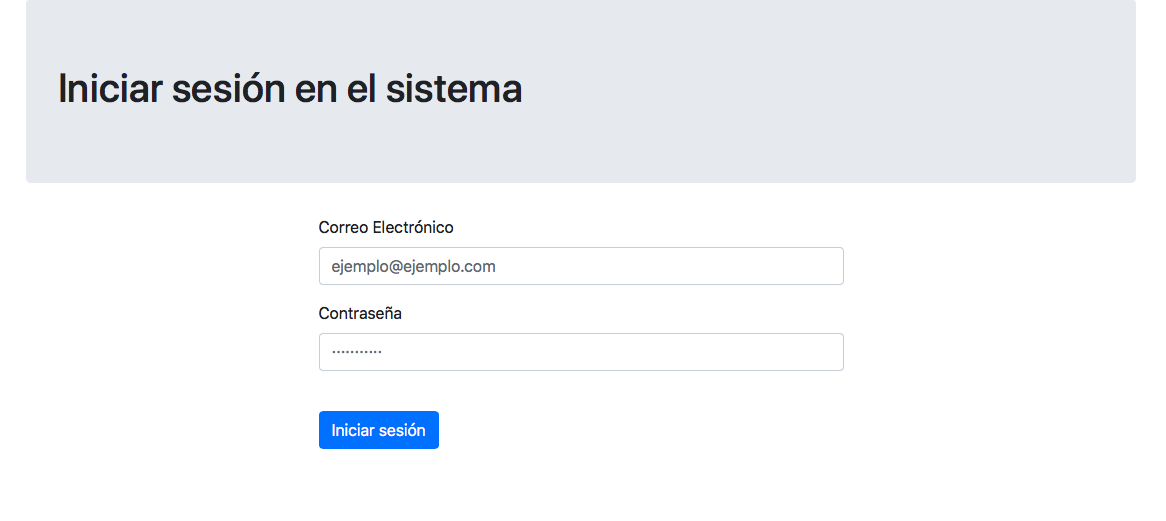
\includegraphics[width=0.9\textwidth]{/captura_login_web.png}
		\caption{Login de la Web}
		\label{fig:login_web}
	\end{center}
\end{figure}

\begin{figure}[!h]
	\begin{center}
		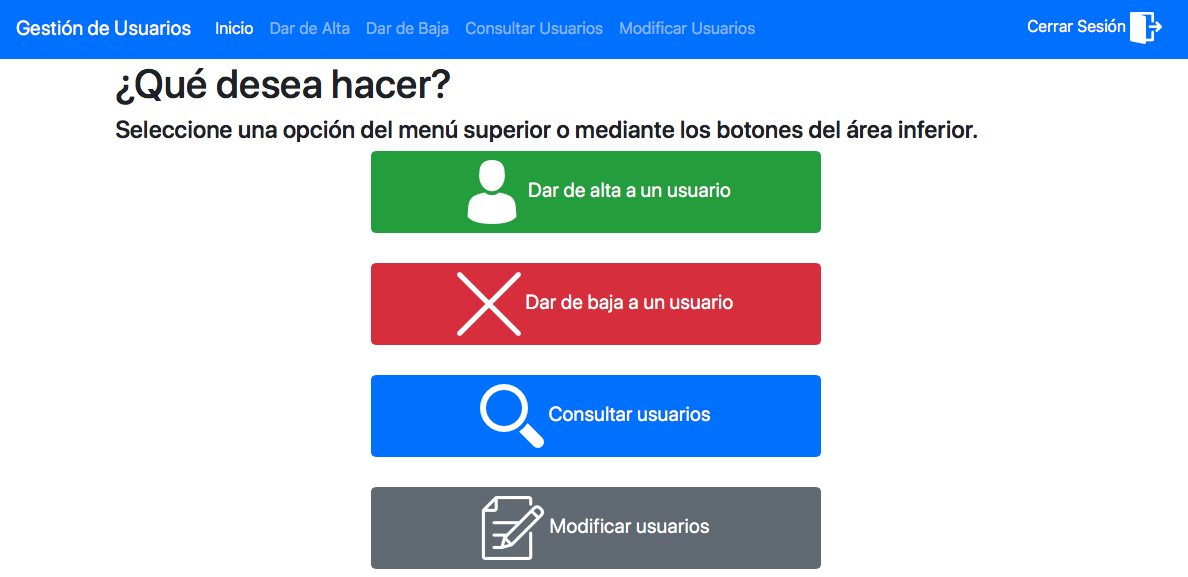
\includegraphics[width=0.9\textwidth]{/captura_index_web.png}
		\caption{Página Principal de la Web}
		\label{fig:index_web}
	\end{center}
\end{figure}

\newpage

\noindent \underline{Dar de Alta} \newline
En esta primera funcionalidad, el administrador tiene la opción de rellenar un formulario para introducir un nuevo usuario en la base de datos, en el que se pueden incluir los datos de un único tutor legal del alumno o, si lo hubiese, también con los del segundo tutor. Los datos que se han especificado para cada tutor son: nombre, primer apellido, segundo apellido, número de teléfono y correo electrónico. Por último, para identificar a este usuario en la base de datos, se le asignará un identificador compuesto del primer apellido de ambos tutores o, en su defecto, del único tutor, añadiendo un número al final. Es decir, si dos familias diferentes poseen los mismos apellidos, se añadirá un número al final de la composición de sus apellidos para el identificador, por lo que quedarán representadas de manera única en la base de datos. Por otra parte, además de disponer del formulario para introducir nuevos usuarios, el administrador también tiene la posibilidad de importar un archivo \acs{CSV} para realizar esta tarea de una manera más sencilla y automatizada. Este archivo debe tener un formato específico detallado en la primera línea del mismo y que consta, principalmente, de los mismos datos que en el formulario pero separados por comas y sin espacios entre ellos, separando los usuarios por un salto de línea.

\noindent \underline{Dar de Baja} \newline
Al entrar en esta página, se dispone de una lista desplegable en la que se cargarán todos los usuarios registrados en la base de datos Web. Al seleccionar uno de ellos, automáticamente se cargarán en una tabla los datos del mismo. Como medida adicional contra el borrado accidental, la página pedirá al usuario que confirme la acción solicitada antes de ser llevada a cabo.

\noindent \underline{Consultar Usuarios} \newline
De manera similar, se ha implementado una tabla para consultar los datos de los usuarios aunque, en este caso, se dispone de una herramienta básica de búsqueda en la que se puede filtrar por cada uno de los campos existentes en la base de datos. Si se pulsa el botón de buscar sin escribir nada en el filtro, la tabla se cargará con todos los registros existentes.

\noindent \underline{Modificar Usuarios} \newline
Esta funcionalidad se ha implementado mediante el uso de una lista desplegable que carga todos los usuarios de la base de datos y un formulario que inicialmente se muestra bloqueado para prevenir una modificación accidental de los datos. Al seleccionar uno de estos usuarios, su información se carga en el formulario y al pinchar el botón de modificar se habilitan los campos para la escritura. Cuando el administrador finalice la modificación de la información, deberá hacer click de nuevo en un botón para terminar la modificación, siendo preguntado sobre si realmente desea llevarla a cabo. En caso positivo, se sobreescribirá la información del usuario seleccionado de la base de datos.

\section{Sprint 2: Creación de la aplicación Android y creación de chats grupales}
Este Sprint está dedicado íntegramente a la aplicación para dispositivos móviles, con lo que ésto conlleve en cuanto a las tareas de diseño y comunicación con la base de datos. De esta manera, los docentes serán los únicos capaces de crear un grupo y las familias podrán ver todos los grupos a los que han sido añadidas. También cada uno de los usuarios será capaz de enviar mensajes que aparecerán en el grupo acompañados de su nombre y fecha y hora de envío.

\newpage

\subsection{Planificación del Sprint}
Para este segundo Sprint se han seleccionado las siguientes historias de usuario:

\begin{table}[hp]
	\centering
	{\small
		\resizebox{15cm}{!} {
	\begin{tabular}{|l|l|}
		\hline
		\multicolumn{2}{|c|}{\cellcolor[HTML]{343434}{\color[HTML]{FFFFFF} \textbf{Historia de Usuario}}} \\
		\hline
		\multicolumn{2}{|c|}{\textbf{Sprint Asignado:} 3.} \\
		\hline
		\textbf{Número de Historia:} 5. & \textbf{Usuario/Rol:} Docente.\\
		\hline
		\multicolumn{2}{|l|}{\textbf{Nombre de la Historia:} Análisis del tono de los mensajes.} \\
		\hline
		\textbf{Prioridad:} Alta. & \textbf{Duración:} 4 horas.\\
		\hline
		\multicolumn{2}{|l|}{\textbf{Descripción:} Analizar el tono de los mensajes de los usuarios y mostrarlos al administrador del chat.} \\
		\hline
		\specialcell{\textbf{Tareas:} Creación e integración \\ de los servicios de IBM Bluemix. \\ Mostrar al administrador de chat \\ los tonos de cada mensaje y usuario.} & \textbf{Pruebas:} \\
		\hline
	\end{tabular}
}






%\begin{tabular}{| c | c | c | c | c | c |}
%	\hline
%	\multicolumn{6}{|c|}{\cellcolor[HTML]{000000}{\color[HTML]{FFFFFF} \textbf{Historia de Usuario}}} \\ 
%	\hline \multicolumn{6}{|c|}{\textbf{Sprint Asignado:} 1} \\
%	\hline \multicolumn{3}{|l|}{\textbf{Número de Historia:} 1} & \multicolumn{3}{l|}{\textbf{Usuario/Rol:} Administrador} \\
%	\hline \multicolumn{6}{|l|}{\textbf{Nombre de la Historia:} Gestión de usuarios de la aplicación móvil} \\
%	\hline \multicolumn{3}{|l|}{\textbf{Prioridad:} Alta} & \multicolumn{3}{l|}{\textbf{Duración:} 30 horas} \\
%	\hline \multicolumn{6}{|l|}{\textbf{Descripción:} Desarrollar una plataforma Web para facilitar la gestión de los usuarios de la aplicación móvil.} \\
%	\hline \multicolumn{6}{|l|}{\textbf{Tareas:}} \\
%	\hline
%\end{tabular}

% Local variables:
%   coding: utf-8
%   ispell-local-dictionary: "castellano8"
%   TeX-master: "main.tex"
% End:

	}
	\caption[Historia de Usuario 2]
	{Historia de Usuario 2}
	\label{tab:historia2}
\end{table}

\begin{table}[hp]
	\centering
	{\small
		\resizebox{15cm}{!} {
	\begin{tabular}{|l|l|}
		\hline
		\multicolumn{2}{|c|}{\cellcolor[HTML]{343434}{\color[HTML]{FFFFFF} \textbf{Historia de Usuario}}} \\
		\hline
		\multicolumn{2}{|c|}{\textbf{Sprint Asignado:} 2.} \\
		\hline
		\textbf{Número de Historia:} 3. & \textbf{Usuario/Rol:} Docente.\\
		\hline
		\multicolumn{2}{|l|}{\textbf{Nombre de la Historia:} Creación de chats grupales.} \\
		\hline
		\textbf{Prioridad:} Alta. & \textbf{Duración:} 10 horas.\\
		\hline
		\multicolumn{2}{|l|}{\textbf{Descripción:} Proporcionar al docente un método de crear un nuevo chat.} \\
		\hline
		\specialcell{\underline{\textbf{Tareas}} \\ Adecuación de la estructura de la base de datos. \\ Diseño de la actividad de creación de grupos.} & \specialcell{\underline{\textbf{Pruebas}} \\ Correcta creación del chat en la nueva colección. \\ Comprobar que se elige un nombre del chat válido. \\ Comprobar que se elige, al menos, una familia.} \\
		\hline
	\end{tabular}
}


	}
	\caption[Historia de Usuario 3]
	{Historia de Usuario 3}
	\label{tab:historia3}
\end{table}

\begin{table}[hp]
	\centering
	{\small
		\resizebox{15cm}{!} {
	\begin{tabular}{|l|l|}
		\hline
		\multicolumn{2}{|c|}{\cellcolor[HTML]{343434}{\color[HTML]{FFFFFF} \textbf{Historia de Usuario}}} \\
		\hline
		\multicolumn{2}{|c|}{\textbf{Sprint Asignado:} 2.} \\
		\hline
		\textbf{Número de Historia:} 5. & \textbf{Usuario/Rol:} Docente, Familia.\\
		\hline
		\multicolumn{2}{|l|}{\textbf{Nombre de la Historia:} Envío y recepción de mensajes de un determinado chat.} \\
		\hline
		\textbf{Prioridad:} Alta. & \textbf{Duración:} 8 horas.\\
		\hline
		\multicolumn{2}{|l|}{\textbf{Descripción:} Añadir capacidad de poder enviar y leer mensajes de los chats de los que se es miembro.} \\
		\hline
		\specialcell{\underline{\textbf{Tareas}} \\ Diseño de la actividad principal. \\ Diseño de la actividad de grupo.} & \specialcell{\underline{\textbf{Pruebas}} \\ Únicamente se muestran chats de los que se es miembro. \\ Carga de chats al iniciar la aplicación. \\ Carga de mensajes al abrir el chat. \\ Desplazamiento al último mensaje cuando se recibe uno nuevo.} \\
		\hline
	\end{tabular}
}

	}
	\caption[Historia de Usuario 4]
	{Historia de Usuario 4}
	\label{tab:historia4}
\end{table}

\newpage

\subsection{Resultados del Sprint}
\subsubsection{Diseño de la actividad de acceso}
Esta tarea requiere de la integración previa de Firebase con la aplicación Android, por lo que se han seguido los pasos necesarios indicados por la propia herramienta para que dicha aplicación pueda comunicarse con los servicios que ofrece la plataforma de Google. Una vez hecho esto, se procede a diseñar la actividad de acceso desde la que los usuarios podrán identificarse en el sistema antes de poder visualizar o enviar mensajes al mismo. Desde un primer momento se ha separado la identificación de los usuarios mediante un \textit{login} <<normal>> y otro específico para docentes, que se muestra mediante un botón independiente, como se puede ver en la Figura \ref{fig:login1}.

\begin{figure}[!h]
	\begin{center}
		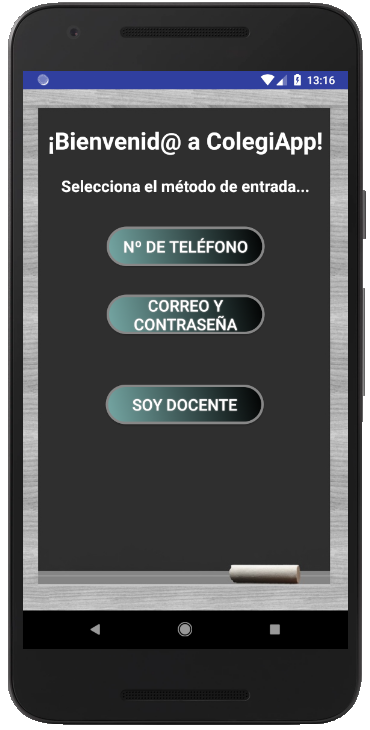
\includegraphics[width=0.4\textwidth]{/capturas_app/login1.png}
		\caption{Actividad inicial}
		\label{fig:login1}
	\end{center}
\end{figure}

\newpage

En el caso de seleccionar el número de teléfono como método de entrada, la aplicación preguntará por un número de teléfono (Figura \ref{fig:logintfno}) al usuario, comprobará su existencia en la base de datos y, si el resultado es positivo, se le mandará un mensaje vía SMS con un código que se debe introducir antes de 60 segundos para que el sistema pueda registrar al usuario mediante Firebase \textit{Authentication}.

\begin{figure}[!h]
	\begin{center}
		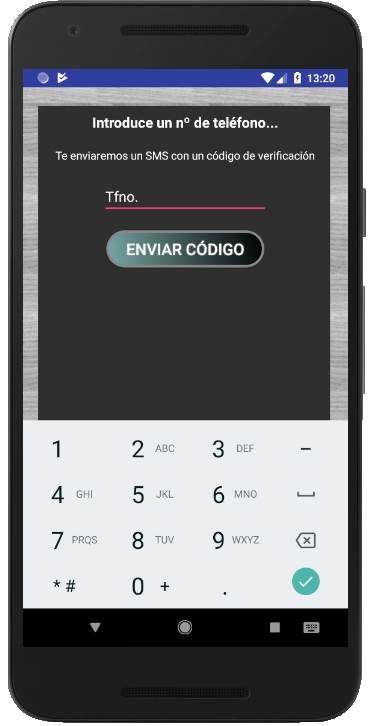
\includegraphics[width=0.4\textwidth]{/capturas_app/logintfno.png}
		\caption{Actividad \textit{login} con teléfono}
		\label{fig:logintfno}
	\end{center}
\end{figure}

Por el contrario, si el usuario decide entrar a la aplicación mediante un correo electrónico y una contraseña, éste deberá introducir ambos campos (Figura \ref{fig:logincorreo}) y, de nuevo, se realizará una primera comprobación de su existencia en la base de datos. En caso de que sea la primera vez que se accede a la aplicación no tendrá contraseña asignada, por lo que la contraseña que se introduzca por primera vez será la que el sistema utilizará para su identificación en futuras ocasiones.

\begin{figure}[!h]
	\begin{center}
		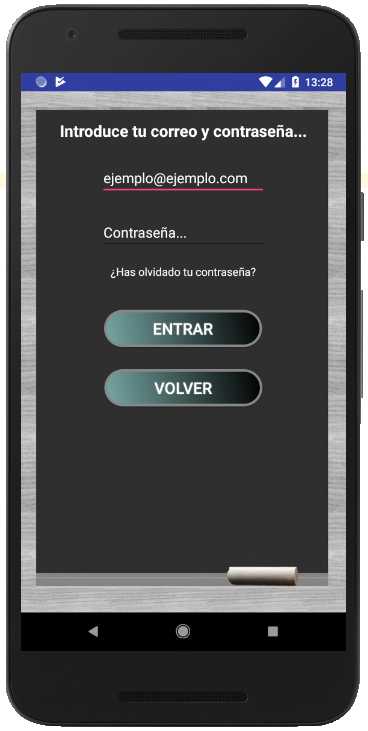
\includegraphics[width=0.4\textwidth]{/capturas_app/logincorreo.png}
		\caption{Actividad \textit{login} con correo y contraseña}
		\label{fig:logincorreo}
	\end{center}
\end{figure}

\newpage

Si el usuario no recuerda su contraseña o decide cambiarla, podrá hacerlo mediante la función <<¿Has olvidado tu contraseña?>>, en la que deberá introducir su correo y, acto seguido, el sistema enviará un correo de recuperación a la dirección indicada siempre que ésta se encuentre en la base de datos. El mensaje contendrá una dirección Web a la que el usuario debe ir para introducir su nueva contraseña (Figura \ref{fig:cambiopass}). Una vez finalizado el proceso, podrá acceder al sistema con su nueva clave.

\begin{figure}[!h]
	\begin{center}
		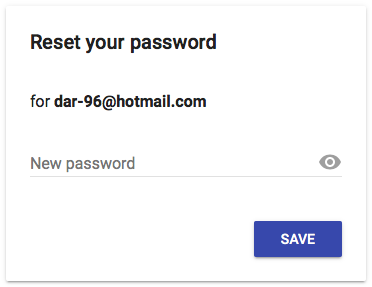
\includegraphics[width=0.3\textwidth]{/capturas_app/cambiopass.png}
		\caption{Cambio de contraseña}
		\label{fig:cambiopass}
	\end{center}
\end{figure}

\clearpage

Por otra parte, si quien quiere acceder a la aplicación es un docente, éste deberá seleccionar la opción <<Soy Docente>>, en cuyo caso se preguntará si quiere autenticarse mediante número de teléfono o mediante correo y contraseña (Figura \ref{fig:logindocente})

\begin{figure}[!h]
	\begin{center}
		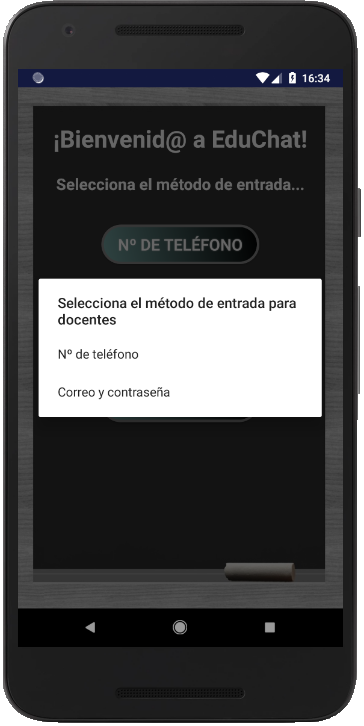
\includegraphics[width=0.35\textwidth]{/capturas_app/logindocente.png}
		\caption{Autenticación docente}
		\label{fig:logindocente}
	\end{center}
\end{figure}

\subsubsection{Adecuación de la base de datos}
A la hora de guardar los grupos de chat se debe crear una nueva colección en la base de datos con todos los datos de los mismos cuyo nombre es <<ChatsGrupales>>. En esta colección se encuentra un documento <<Control>> con un campo <<Contador>>, que se trata de un número entero usado para otorgar un identificador único a cada una de las salas de chat en la base de datos y que se irá incrementando a medida que se vayan creando nuevos grupos. Cada uno de ellos contendrá un objeto de tipo <<Administrador>>, que será el docente creador del grupo con todos sus datos; su identificador en la base de datos y el nombre que el docente haya asignado a dicho grupo. Además, contendrá dos colecciones adicionales: <<Familias>> y <<Mensajes>>. La primera incluye los documentos de la colección <<Usuarios>> que el administrador haya incluido en el grupo, es decir, las familias participantes. Por su parte, la colección <<Mensajes>>, incluye documentos con los mensajes que cada integrante ha enviado al grupo, conteniendo cada uno el nombre, apellidos, correo electrónico o teléfono con el que el usuario se identificó, la fecha de envío y, finalmente, el mensaje.

\subsubsection{Diseño de la actividad de creación de grupos}
Una vez que el docente se ha identificado en el sistema y ha accedido a la actividad principal, podrá crear un nuevo grupo mediante la opción <<Crear grupo>> situada en el menú principal de la aplicación, que se encuentra en el borde superior derecho de la pantalla. Al seleccionar esta opción, se mostrará una nueva actividad en la que se podrá introducir el nombre del grupo y los integrantes del mismo (Figura \ref{fig:creargrupo}) mediante una lista en la que se cargarán todas las familias que se encuentren en ese momento en la colección <<Usuarios>>. Para finalizar su creación, se debe pulsar el botón <<Crear Grupo>>, en cuyo caso la aplicación preguntará al docente si realmente desea crear ese grupo y se le devolverá a la actividad principal, donde se muestran los grupos de los que el usuario es miembro.

\begin{figure}[!h]
	\begin{center}
		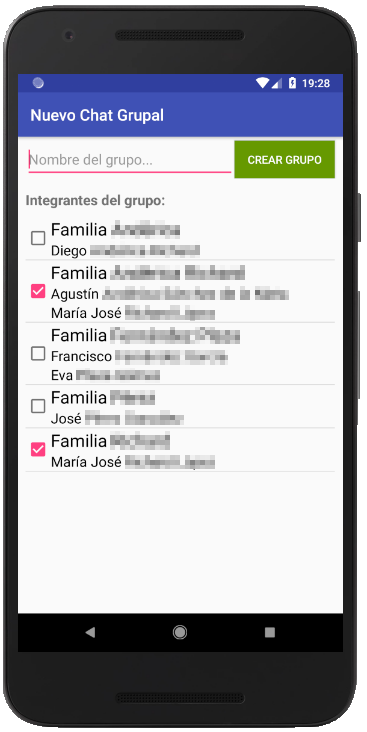
\includegraphics[width=0.4\textwidth]{/capturas_app/creargrupo.png}
		\caption{Actividad Crear Grupo}
		\label{fig:creargrupo}
	\end{center}
\end{figure}

\newpage

\subsubsection{Diseño de la actividad principal}
Esta actividad será la primera que el usuario visualice nada más entrar a la aplicación y, por tanto, su principal función reside en mostrar una lista con los grupos de chat de los que sea miembro. Dicha aplicación se conectará a la base de datos y buscará en la colección <<Familias>> de cada uno de los documentos de chats de la colección <<ChatsGrupales>> para comprobar su pertenencia a los mismos. Durante este proceso se mostrará al usuario un diálogo de carga que, una vez completada la tarea de búsqueda, mostrará la lista ya cargada con todos los grupos a los que se tiene acceso y en los que el usuario podrá pinchar para acceder a ellos, abriendo la actividad responsable de mostrar los mensajes.

\subsubsection{Diseño de la actividad de grupo}
Por último, la principal función de la actividad de grupo es la de mostrar todos los mensajes que se han ido mandando desde su creación. En este caso, a diferencia de la actividad principal, donde se ha implementado una \textit{ListView}, en la actividad de grupo se ha utilizado una \textit{RecyclerView} (Figura \ref{fig:listview}) pensando en la eficiencia de la aplicación. Una \textit{RecyclerView} es una lista en la que se <<reciclan>> las filas de ésta cuando el usuario se desplaza hacia arriba o hacia abajo y no se están mostrando. Por tanto, el rendimiento aumenta al tener muchas filas o, en este caso, mensajes en un grupo.

\begin{figure}[!h]
	\begin{center}
		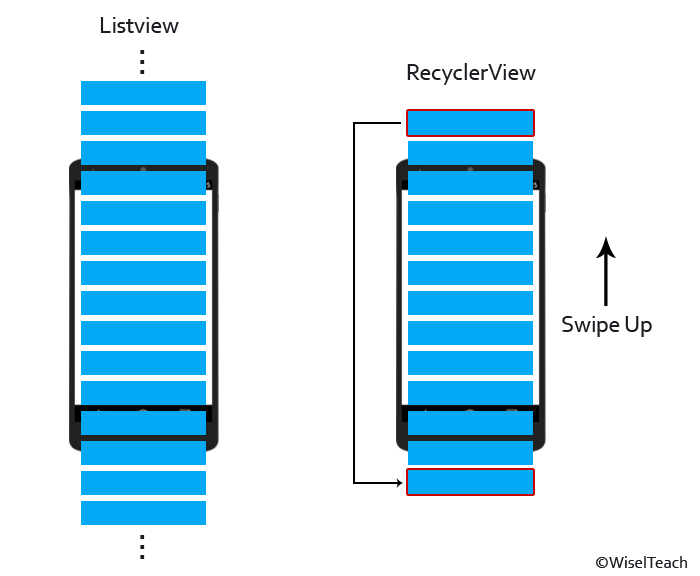
\includegraphics[width=0.5\textwidth]{/listview.png}
		\caption{\textit{ListView} vs \textit{RecyclerView}}
		\label{fig:listview}
	\end{center}
\end{figure}